\chapter{Proposed Framework}
\label{ch:Framework}

A real case application would probably have several signals of several phisical quantities, so a general approach that can manage different types of features, and extract from each of them the most relevant information, is needed.

\begin{figure}
    \centering
    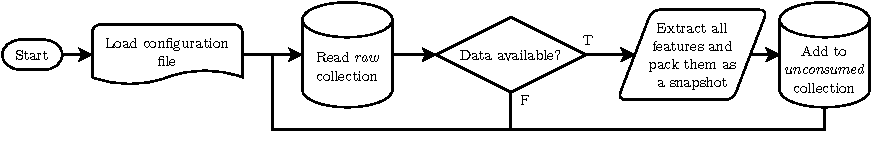
\includegraphics[width=\textwidth]{images/Framework/FA_flowchart.pdf}
    \caption{Feature Agent flowchart}
    \label{fig:FA_flowchart}
\end{figure}

\begin{figure}
    \centering
    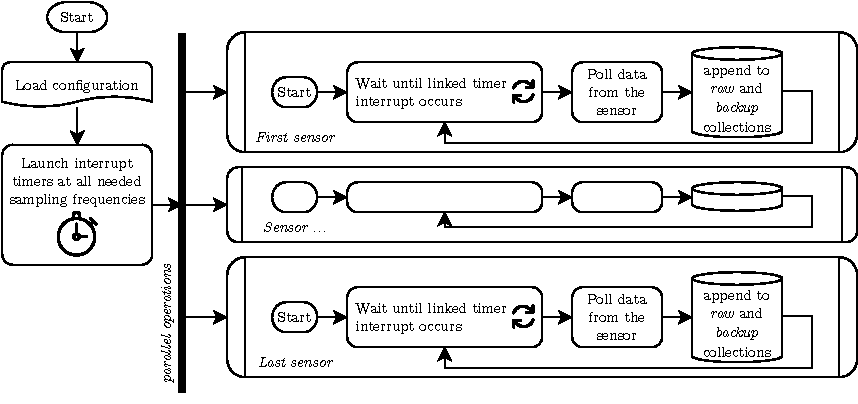
\includegraphics[scale=1]{images/Framework/Field_Agent_flowchart.pdf}
    \caption{Field Agent flowchart}
    \label{fig:Field_Agent_flowchart}
\end{figure}

\begin{figure}
    \centering
    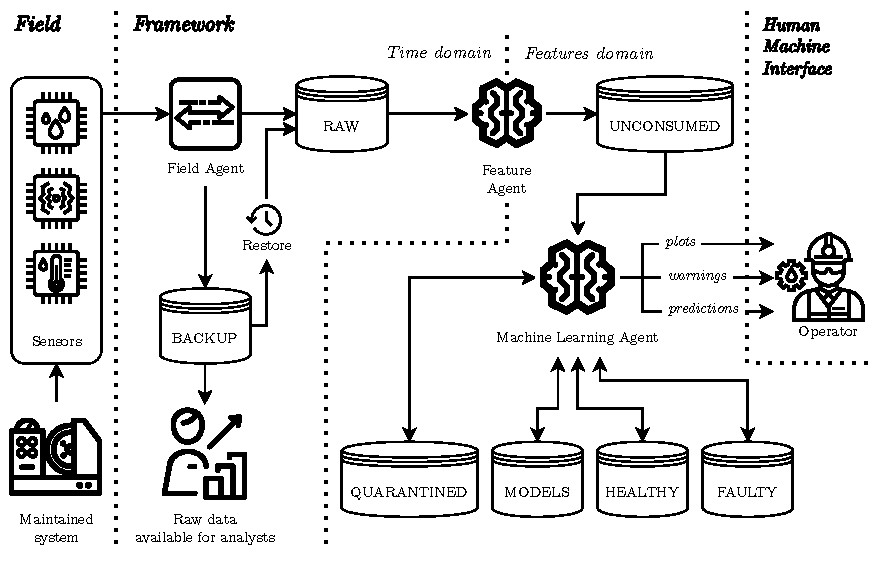
\includegraphics[width=\textwidth]{images/Framework/Framework_structure.pdf}
    \caption{Framework locical structure}
    \label{fig:Framework_structure}
\end{figure}

\begin{figure}
    \centering
    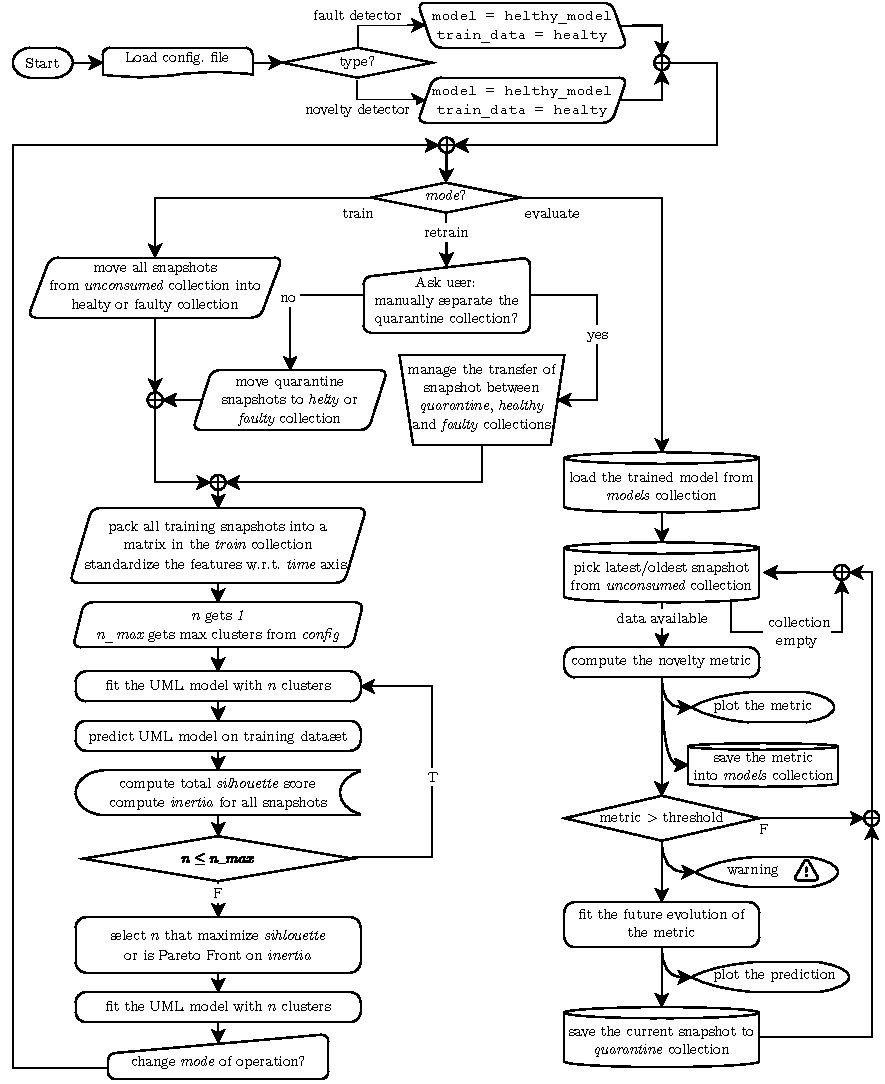
\includegraphics[width=\textwidth]{images/Framework/MLA.pdf}
    \caption{Machine Learning Agent flowchart. When it is instanced for \gls{nd}, the \gls{mla} uses the healthy collection as training dataset, when it is instanced for \gls{fd} it uses the faulty collection.}
    \label{fig:MLA_structure}
\end{figure}


